\documentclass[manual-fr.tex]{subfiles}
\begin{document}

Once launched, the user needs to select the following things:
\begin{itemize}
    \item data used for training;
    \item the workflow to preprocess data.
\end{itemize}

~

To select the data that will be used for training, see figures \ref{fig:train_sem-02} and \ref{fig:train_sem-03}. The different steps are :
\begin{enumerate}
    \item click on the \emph{select file(s)} button;
    \item select annotated files;
    \item click on the \emph{open} button.
\end{enumerate}

~

When they are selected, files will be listed as shown in figure \ref{fig:train_sem-03}. It is not necessary that selected files have the same format. They can have any format that is readable by SEM. Currently, the supported formats are:
\begin{itemize}
    \item XML SEM, the internal XML format of SEM;
    \item json SEM, the internal json format of SEM;
    \item BRAT \cite{stenetorp2012brat};
    \item GATE \cite{cunningham2002gate};
\end{itemize}

~

When annotated files are selected, a workflow has to be selected before processing documents. SEM offer an example of a workflow to retrain NER in figure \ref{fig:train_sem-02}: \emph{NER-train.xml}.

\begin{figure}[ht!]
    \begin{center}
    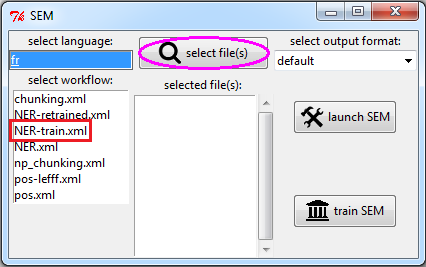
\includegraphics[scale=0.5]{fr/images/train_sem-02.png}
    \end{center}
    \caption{Circled in purple : the button to select documents for training. Framed in red : the workflow to use to train models.}
    \label{fig:train_sem-02}
\end{figure}

\begin{figure}[ht!]
    \begin{center}
    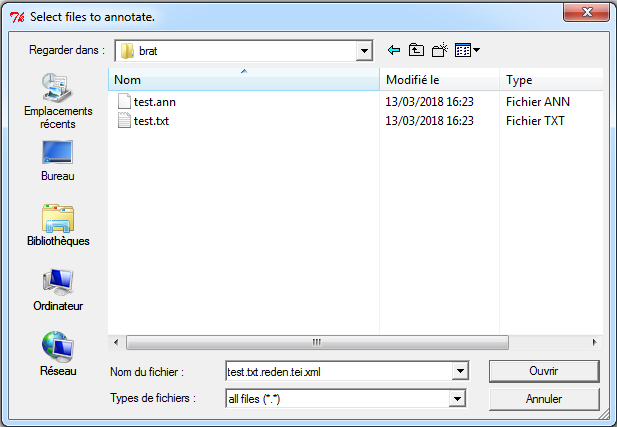
\includegraphics[scale=0.5]{fr/images/train_sem-03.png}
    \end{center}
    \caption{Examples of annotated files in BRAT format. Select ".ann" or ".txt" for training.}
    \label{fig:train_sem-03}
\end{figure}

\begin{figure}[ht!]
    \begin{center}
    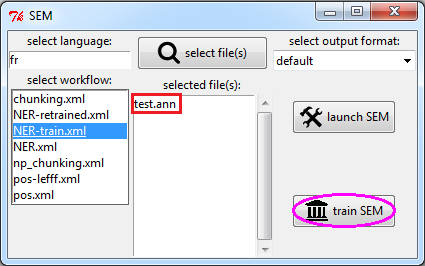
\includegraphics[scale=0.5]{fr/images/train_sem-04.png}
    \end{center}
    \caption{framed in red : documents used for training. Circled in purple : the button to retrain SEM.}
    \label{fig:train_sem-04}
\end{figure}

\end{document}
